\documentclass[a4paper]{report}

\usepackage[utf8]{inputenc}
\usepackage[english]{babel}
\usepackage[T1]{fontenc}
\usepackage{textcomp}
\usepackage[]{amsthm} 
\usepackage[]{amssymb}
\usepackage{graphicx}
\usepackage{float}
\usepackage{soul}
\usepackage{color}
\usepackage{bm}
\usepackage{listings}
\usepackage{xcolor}
\usepackage{enumitem}
%\usepackage{xfrac}
\usepackage[normalem]{ulem}

% ~~~~ no indent per paragraph ~~~~-
\usepackage[parfill]{parskip}

% ~~~~ hyperlinks ~~~~ 
\usepackage[colorlinks=true, linkcolor=blue]{hyperref}

% ~~~~ subfigs ~~~~
\usepackage{subcaption}

% ~~~~ math ~~~~
\usepackage{amsmath}

\usepackage{mathtools}
% ~~ colorbox : "align" use only ~~
\newcommand{\myboxA}[1]{
	\fcolorbox{black}{lime}{#1}
}
\MakeAboxedCommand\AboxedA\myboxA

% ~~ colorbox : else ~~
\newcommand{\mybox}[1]{
	\fcolorbox{black}{lime}{$\displaystyle#1$}
}

% ~~~~ graphics ~~~~
\usepackage{tikz}
\usetikzlibrary{trees}
\usetikzlibrary {fit,shapes.geometric} % W: Command terminated with space. (1)
\usetikzlibrary {automata} % W: Command terminated with space. (1)
\usetikzlibrary{arrows.meta}
\usepackage{multicol}

\usepackage{pgfplots}
\pgfplotsset{compat = newest}

\usepackage{geometry}
\geometry{legalpaper, margin=1in}

% ~~~~ upgraded tables ~~~~
\usepackage{booktabs}

% ~~~~ algorithm formatting ~~~~
\usepackage{algorithm}
\usepackage[noend]{algpseudocode}
\usepackage{caption}

% ~~~~ list bullets ~~~~
\renewcommand{\labelitemii}{$\circ$}
\renewcommand{\labelitemiii}{$\star$}
\renewcommand{\labelitemiv}{$>$}

% figure support
\usepackage{import}
\usepackage{xifthen}
\pdfminorversion=7
\usepackage{pdfpages}
\usepackage{transparent}
\newcommand{\incfig}[1]{%
    \def\svgwidth{\columnwidth}
    \import{./figures/}{#1.pdf_tex}}

% Newline for algorithm psuedo
\newcommand{\algrule}[1][.2pt]{\par\vskip.5\baselineskip\hrule height #1\par\vskip.5\baselineskip}

% -------- Listings/XColor Settings --------
\definecolor{codegreen}{rgb}{0,0.6,0}
\definecolor{codegray}{rgb}{0.5,0.5,0.5}
\definecolor{codepurple}{rgb}{0.58,0,0.82}
\definecolor{backcolour}{rgb}{0.95,0.95,0.92}

\lstdefinestyle{mystyle}{
	backgroundcolor=\color{backcolour},
	commentstyle=\color{codegreen},
	keywordstyle=\color{magenta},
	numberstyle=\tiny\color{codegray},
	stringstyle=\color{codepurple},
	basicstyle=\ttfamily\scriptsize,
	breakatwhitespace=false,
	breaklines=true,
	captionpos=b,
	keepspaces=true,
	numbers=left,
	numbersep=5pt,
	showspaces=false,
	showstringspaces=false,
	showtabs=false,
	tabsize=4
}

\lstset{style=mystyle}

% -------------- Doc Start -------------------



\pdfsuppresswarningpagegroup=1

\title{\Huge{Trade Study of Pipelined 32-bit  Ripple Carry Adder}}
\author{\textbf{Authors:} \\WhisperingRock\\}
\date{\today}

\begin{document}
    \maketitle

	\chapter{Timing Analysis}

		Variables used to explain timing:
		\begin{itemize}
			\item $n$: the number of full adders. Also the number of bits
				added. 
			\item $t_{dFA}$: the worst case carry propagation
				delay through one FullAdder module.
			\item $t_{reg}$: delay for register CLK-to-Q and setup.
			\item $t_{skew}$: clock skew and timing margin.
			\item $k$: the number of pipeline stages.
		\end{itemize}

		\section{RippleCarryAdder}
			The combination logic \texttt{RippleCarryAdder} doesn't have a 
			clock signal so we must only consider the propagation variable
			$t_{dFA}$. 

			Since there are 8 bits propagated in sequence, each RCA has a 
			summation delay of
			 \[
				 t_{dRCA} = 8 \cdot t_{dFA}
			\] 
			
			The \textbf{latency} of the RCA is our sequential propagation. 
			\[
				L_{RCA} = t_{dRCA}
			\] 

			The \textbf{throughput} of the RCA is
			\[
				\text{Throughput}_{RCA} = \frac{1}{L_{RCA}}
			\] 

			\begin{figure}[H]
				\centering
				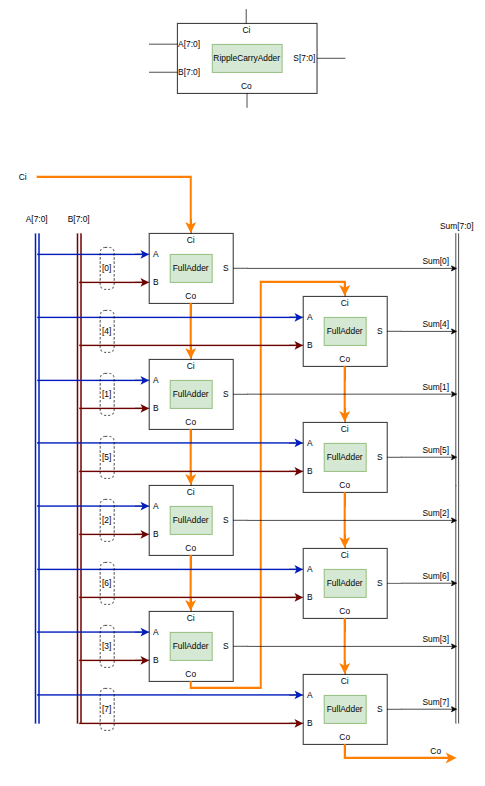
\includegraphics[
					width			= 0.8\textwidth,
					keepaspectratio	= true
					]{./pics/rca_block.png}
				\caption{Block Diagram of the 8-bit RippleCarryAdder}
				\label{fig:rca-block}
			\end{figure}

			\begin{figure}[H]
				\centering
				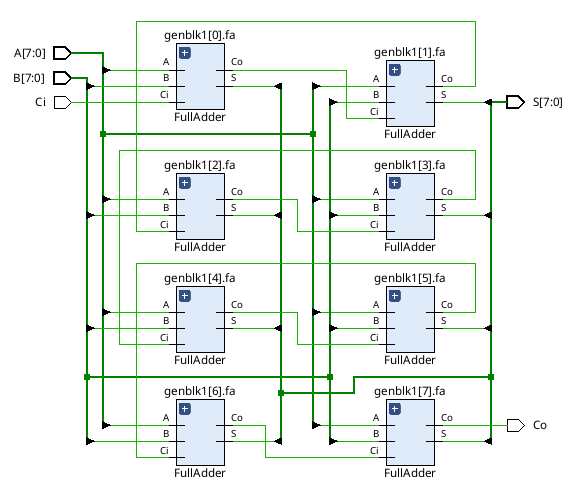
\includegraphics[
					width			= 0.8\textwidth,
					keepaspectratio	= true
					]{./pics/rca_rtl.png}
				\caption{RTL of the 8-bit RippleCarryAdder}
				\label{fig:rca-rtl}
			\end{figure}

			Code for RCA and test are \ref{code:rca} and \ref{testcode:rca}.
			Code for the FullAdder and test are \ref{code:fa} and \ref{testcode:fa}.
		

		\newpage
		\section{WordAdder}
			The \texttt{WordAdder} is four RCAs in series due to the carry bit.
			The propagation here is 

			\[
				t_{dWA} = 4 \cdot t_{dRCA} = 32 \cdot t_{dFA}
			\]

			The \textbf{latency} of the WordAdder is our sequential propagation. 
			\[
				\mybox{L_{WA} = t_{dWA} = 32 \cdot t_{dFA}}
			\] 

			The \textbf{throughput} of the WA is
			\[
				\mybox{\text{Throughput}_{WA} = \frac{1}{L_{WA}} = \frac{1}{32 \cdot t_{dFA}}}
			\] 

			\begin{figure}[H]
				\centering
				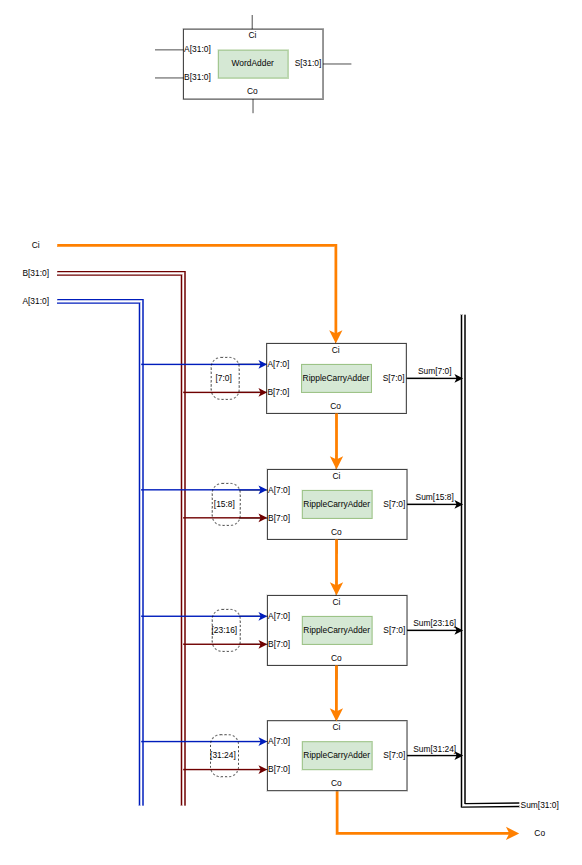
\includegraphics[
					width			= 0.8\textwidth,
					keepaspectratio	= true
					]{./pics/word_block.png}
				\caption{Block Diagram of the 32-bit WordAdder}
				\label{fig:word-block}
			\end{figure}

			\begin{figure}[H]
				\centering
				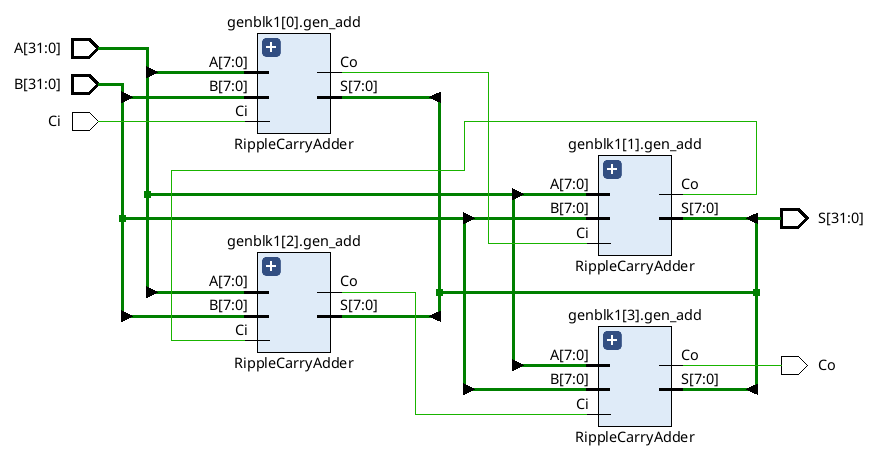
\includegraphics[
					width			= 0.8\textwidth,
					keepaspectratio	= true
					]{./pics/word_rtl.png}
				\caption{RTL of the 32-bit WordAdder}
				\label{fig:word-rtl}
			\end{figure}

			Code for WA and test are \ref{code:word} and \ref{testcode:word}.

		\newpage
		\section{PipedWordAdder}
		
			The piped word adder requires fine-grain calculations. Consider:
			\begin{itemize}
				\item Calculating delays in stages s.t. a single stage must
					sequentially propagate some bits through the FullAdders.
					Here, for our 32-bit word, each of the four stages must
					have time to propagate 8-bits through.
					\[
						t_{stage} \approx \left\lceil \frac{n}{k} \right\rceil t_{dFA} = 8 \cdot t_{dFA}
					\] 
				\item The minimal clock must be greater than the stage delay 
					plus the delays required for clock skew and register storage.
					\[
						T_{CLK,p} \ge t_{stage} + t_{reg} + t_{skew}
					\] 
			\end{itemize}

			Therefore,

			the \textbf{latency} for adding two words together takes four clock cycles, always.
			\[
				\mybox{L_{PWA} = k\cdot T_{CLK,p}}
			\] 

			however, the \textbf{throughput} depends on the vacancy of the pipeline.
			If the pipeline is emptied before processing another pair of words,
			we must wait 4 cycles for an output. If the pipeline was initially full, 
			then 4 results will be output on each clock cycle. Consider:

			\begin{figure}[H]
				\centering
				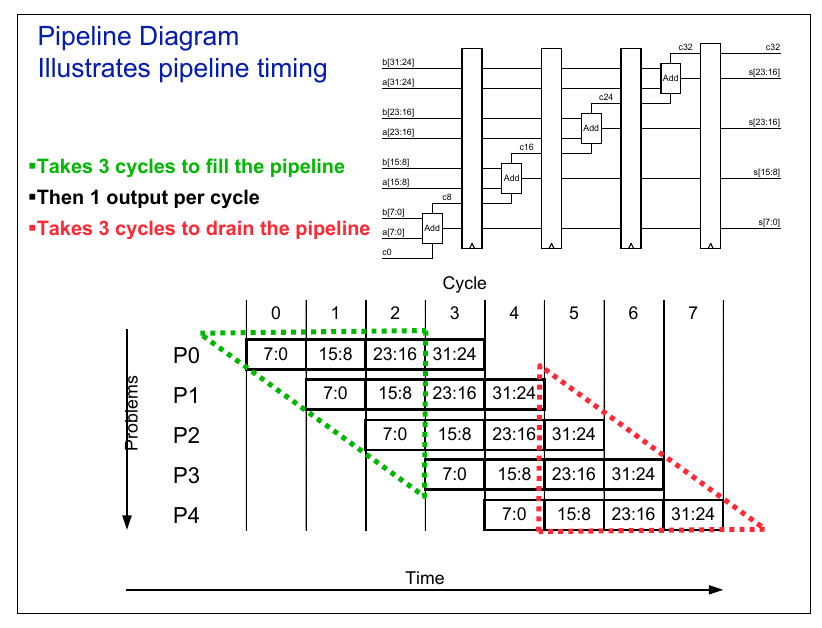
\includegraphics[
					width			= 0.8\textwidth,
					keepaspectratio	= true
					]{./pics/pipefill.png}
				\caption{Filling and Emptying the Pipe}
				\label{fig:pfill}
			\end{figure}

			\[
				\mybox{\text{Throughput}_{PWA}} = 
				\begin{cases*}
					\frac{1}{4\cdot T_{CLK,p}} 	& , if pipe registers are empty \\
					\vdots 						& , \vdots\\
					\frac{1}{T_{CLK,p}}			& , if pipe registers are full
				\end{cases*}
			\] 

			Ideally we have enough work to keep the adder full at all times 
			to utilize the pipeline performance boost.
	
			\begin{figure}[H]
				\centering
				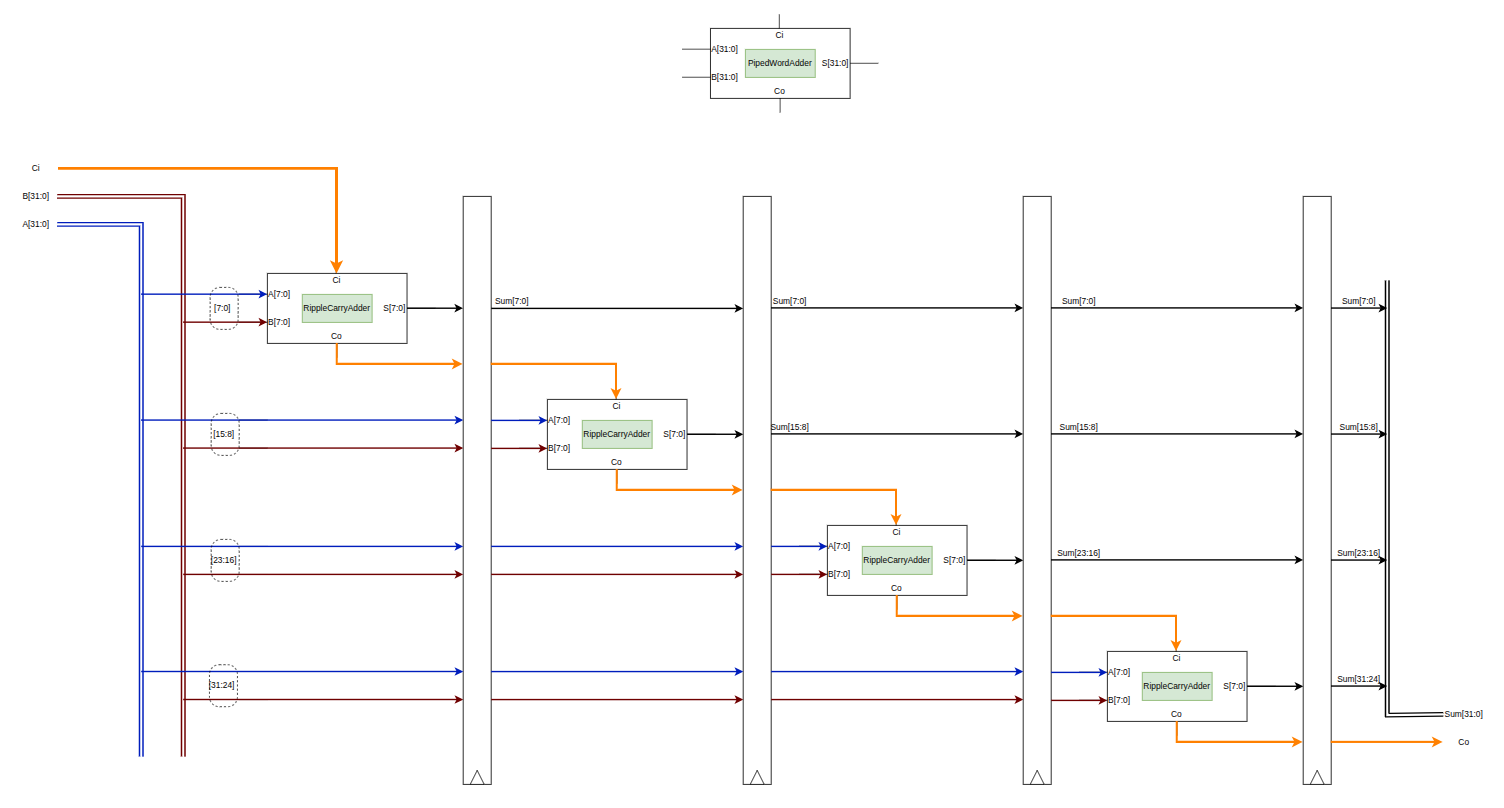
\includegraphics[
					width			= 1.0\textwidth,
					keepaspectratio	= true
					]{./pics/pword_block.png}
				\caption{Block Diagram of the 32-bit Piped WordAdder}
				\label{fig:pword-block}
			\end{figure}

			\begin{figure}[H]
				\centering
				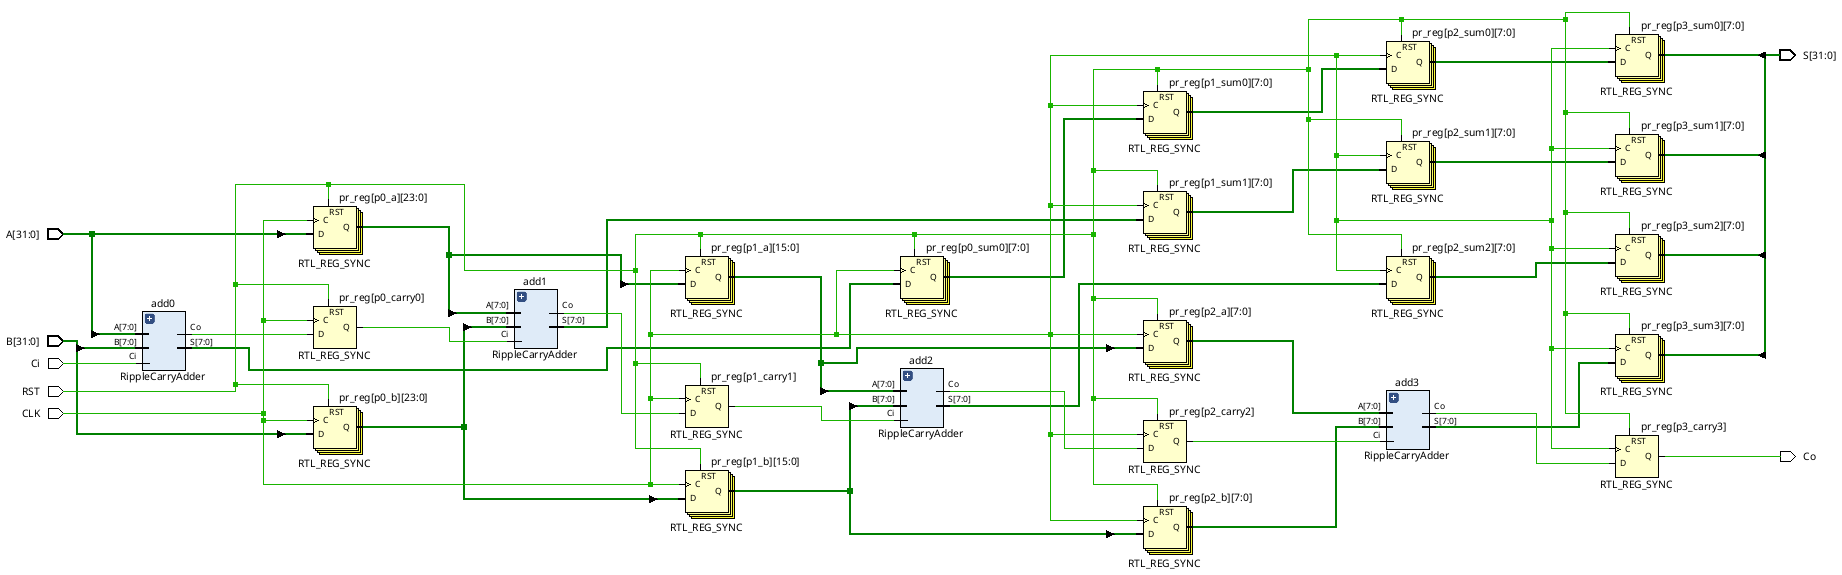
\includegraphics[
					width			= 1.0\textwidth,
					keepaspectratio	= true
					]{./pics/pword_rtl.png}
				\caption{RTL of the 32-bit Piped WordAdder}
				\label{fig:pword-rtl}
			\end{figure}

			Code for PWA and test are \ref{code:pword} and \ref{testcode:pword}.


		\section{Comparison Example}

			Consider an example where
			\begin{itemize}
				\item $n = 32$ bits
				\item $k = 4$ stages
				\item $t_{dFA} = 100 ps$
				\item $t_{reg} = 50 ps$
				\item ignore  $t_{skew}$
			\end{itemize}

			\begin{table}[H]
				\centering
				\begin{tabular}{l c c c}
					\toprule
					 & Non-Pipelined  & Empty Pipeline  & Full Pipeline  \\ 
					\midrule
					Latency(s) 			& 3200p		& $\ge$ 3400p	& $\ge$ 3400p\\
					\midrule
					Throughput(ops/s)	& 312.5 M	& 294 M			& \hl{1,176 M} \\
					\bottomrule
				\end{tabular}
				\caption{Calculation of Pipelined vs. Not Pipelined Ripple Word Adder}
				\label{tab:word}
			\end{table}

			From our simple example, pipelining increases our latency overhead
			by adding in more registers but can greatly increase our throughput
			as long as we can maintain a full pipe. 

			Throughput performance boost $\approx \frac{1176}{312} \approx 3.77 \times$
			
		\newpage
		\section{Testing on hardware}

			I'm skeptical this is possible with the 100MHz Basys3 dev board 
			with current timing estimates for the pipeline in the single-digit 
			nanosecond\ldots \hl{todo}
		
	\newpage
	\chapter{Appendix}

		\section{Design Code}

			\lstinputlisting[
				language 	= {Verilog},
				captionpos	= top, 
				caption		= {\texttt{FullAdder.sv}},
				breaklines	= true, 
				label		= {code:fa}
			]{../00_hardware/00_src/FullAdder.sv}

			\lstinputlisting[
				language 	= {verilog},
				captionpos	= top, 
				caption		= {\texttt{FullAdder\_tb.sv}},
				breaklines	= true, 
				label		= {testcode:fa}
			]{../00_hardware/02_sim/FullAdder_tb.sv}


			\lstinputlisting[
				language 	= {Verilog},
				captionpos	= top, 
				caption		= {\texttt{RippleCarryAdder.sv}},
				breaklines	= true, 
				label		= {code:rca}
			]{../00_hardware/00_src/RippleCarryAdder.sv}

			\lstinputlisting[
				language 	= {verilog},
				captionpos	= top, 
				caption		= {\texttt{RippleCarryAdder\_tb.sv}},
				breaklines	= true, 
				label		= {testcode:rca}
			]{../00_hardware/02_sim/RippleCarryAdder_tb.sv}

			\lstinputlisting[
				language 	= {Verilog},
				captionpos	= top, 
				caption		= {\texttt{WordAdder}},
				breaklines	= true, 
				label		= {code:word}
			]{../00_hardware/00_src/FourAdd.sv}

			\lstinputlisting[
				language 	= {verilog},
				captionpos	= top, 
				caption		= {\texttt{WordAdder\_tb}},
				breaklines	= true, 
				label		= {testcode:word}
			]{../00_hardware/02_sim/FourAdd_tb.sv}


			\lstinputlisting[
				language 	= {Verilog},
				captionpos	= top, 
				caption		= {\texttt{PipedWordAdder}},
				breaklines	= true, 
				label		= {code:pword}
			]{../00_hardware/00_src/FourAdderPipe.sv}

			\lstinputlisting[
				language 	= {verilog},
				captionpos	= top, 
				caption		= {\texttt{PipedWordAdder\_tb}},
				breaklines	= true, 
				label		= {testcode:pword}
			]{../00_hardware/02_sim/FourAdderPipe_tb.sv}

		\section{Utility Code}

			\lstinputlisting[
				language 	= {verilog},
				captionpos	= top, 
				caption		= {Packaged class entities for testing \texttt{tb\_utils\_pkg.sv}},
				breaklines	= true, 
				label		= {code:util}
			]{../00_hardware/02_sim/tb_utils_pkg.sv}
			
\end{document}
